\chapter{Cartesian coordinates}
\label{ch:cartesian}

In this chapter
we apply boundary tracing to the conduction--radiation problem
starting from known solutions
to Laplace's equation~(\ref{eq:laplace-steady-conduction})
in Cartesian coordinates.
Traced boundaries are determined along which
the radiation condition~(\ref{eq:radiation-boundary-condition})
is satisfied;
these are then used to construct conduction--radiation domains
which also admit the known solution.
Two known solutions are analysed here:
the plane-source solution in Section~\ref{sec:cartesian.plane}
and a cosinusoidal solution in Section~\ref{sec:cartesian.cosine}.

\section{Plane-source solution}
\label{sec:cartesian.plane}

First we consider the simplest non-constant solution
to Laplace's equation~(\ref{eq:laplace-steady-conduction})
in Cartesian coordinates,
\begin{important}{equation}
  T = h_0 x,
  \label{eq:plane-laplace-solution}
\end{important}
corresponding to one-dimensional steady conduction
with constant temperature gradient~$h_0$.
Such would be the equilibrium temperature profile in a slab
with one face held at a fixed temperature
and the other radiating into vacuum
(Figure~\ref{fig:plane-slab-bvp}).
The aim of boundary tracing is to look for radiation boundaries
which are more interesting than a straight line (representing a flat face)
but still consistent with the solution~(\ref{eq:plane-laplace-solution}).

\begin{figure}
  \centredfigurecontent[width=0.45\textwidth]{plane-slab-bvp}{
    One-dimensional conduction--radiation problem in a slab.
  }
\end{figure}

In the context of thermal radiation,
the temperature~$T$ is to be reckoned on an absolute scale;
therefore, the region~$x < 0$ is unphysical and ignored,
as the temperature therein is negative.

\subsection{Scaling}
\label{sec:cartesian.plane.scaling}

While the known solution~(\ref{eq:plane-laplace-solution}) is, by itself,
scale-invariant with respect to both temperature and length,
its coupling with
the radiation boundary condition~(\ref{eq:radiation-boundary-condition})
will determine characteristic temperature and length scales
$\Theta$ and~$\lambda$.
Here, we perform scaling to remove these parameters
and reduce the problem to dimensionless form.

Let
\begin{align}
  T &= \Theta \scaled{T}, \label{eq:plane-temperature-scaling} \\
  x &= \lambda \scaled{x}, \label{eq:plane-x-scaling} \\
  y &= \lambda \scaled{y}. \label{eq:plane-y-scaling}
\end{align}
Noting that
\begin{equation}
  \del = \scaleddel / \lambda,
  \label{eq:plane-del-scaling}
\end{equation}
the radiation boundary condition~(\ref{eq:radiation-boundary-condition})
and the known solution~(\ref{eq:plane-laplace-solution})
become
\begin{align}
  \normalvec \dotp \scaleddel \scaled{T}
    &= -\group{c \lambda \Theta^3} \scaled{T}^4,
    \label{eq:plane-scaled-radiation-boundary-condition-with-groups}
    \\[\tallspace]
  \scaled{T}
    &= \group{\frac{h_0 \lambda}{\Theta}} \scaled{x}.
    \label{eq:plane-scaled-laplace-solution-with-groups}
\end{align}
Setting the two dimensionless groups to unity
results in the temperature and length scales
\begin{align}
  \Theta &= \roundbr*{\frac{h_0}{c}}^{1/4},
    \label{eq:plane-temperature-scale} \\[\tallspace]
  \lambda &= \roundbr*{\frac{1}{c {h_0}^3}}^{1/4}.
    \label{eq:plane-length-scale}
\end{align}
These scales may also be arrived at
by seeking the straight-line boundary~$x = \lambda$
and its corresponding temperature~$T = \Theta$
along which the radiation condition~(\ref{eq:radiation-boundary-condition})
is satisfied.
Since the temperature gradient
for the known solution~(\ref{eq:plane-laplace-solution})
is $h_0$~everywhere,
there must hold~$h_0 = c T^4$ along this boundary,
and the scales~(\ref{eq:plane-temperature-scale})
and~(\ref{eq:plane-length-scale}) follow immediately.

Of course the straight-line boundary~$x = \lambda$
(or equivalently~$\scaled{x} = 1$)
is rather boring,
and it is through boundary tracing
that more interesting boundaries may be generated,
as will be shown in the next section.

\subsection{Boundary tracing}
\label{sec:cartesian.plane.tracing}

For brevity we drop all \scalingmarks{}
so that the scaled boundary condition~%
  (\ref{eq:plane-scaled-radiation-boundary-condition-with-groups})
and the known solution~(\ref{eq:plane-scaled-laplace-solution-with-groups})
become
\begin{important}{align}
  \normalvec \dotp \del T &= -T^4,
    \label{eq:plane-scaled-radiation-boundary-condition} \\
  T &= x.
    \label{eq:plane-scaled-laplace-solution}
\end{important}
The scale factors for Cartesian coordinates are trivial
($\scalefac[x] = \scalefac[y] = 1$),
leading to the following abbreviatory quantities
from Section~\ref{sec:curvilinear.derivative.abbreviations}:
\begin{align}
  P &= \pder{T}{x} = 1,
    \label{eq:plane-gradient-x-component} \\[\tallspace]
  Q &= \pder{T}{y} = 0.
    \label{eq:plane-gradient-y-component}
\end{align}
Comparing the radiation boundary condition~%
  (\ref{eq:plane-scaled-radiation-boundary-condition})
to the generic~(\ref{eq:flux-boundary-condition}),
the flux function is
\begin{equation}
  F = -T^4 = -x^4,
  \label{eq:plane-flux-function}
\end{equation}
and it follows that the viability function is
\begin{align*}
  \Phi
  &= (\del T)^2 - F^2 \\
  &= 1 - x^8.
    \yesnumber
    \label{eq:plane-viability-function}
\end{align*}
Traced boundaries will only exist in the viable domain~$\Phi \ge 0$,
which, excluding the unphysical region~$x < 0$,
consists of the infinite strip~$0 \le x \le 1$.

The terminal curve~$\Phi = 0$ is also the $T$-contour~$x = 1$
(the boring traced boundary
mentioned in Section~\ref{sec:cartesian.plane.scaling}).
Using the terminology of Section~\ref{sec:introduction.tracing},
$x = 1$~is therefore a critical terminal curve,
and other traced boundaries will attach to it smoothly.

\begin{figure}
  \centredfigurecontent[width=0.45\textwidth]{%
    plane-traced-boundaries%
  }{
    Traced boundaries~(\ref{eq:plane-traced-boundary}).
  }
\end{figure}

The boundary tracing ODE~(\ref{eq:tracing-ode-coordinate-parametrisation-v})
becomes
\begin{important}{equation}
  \tder{y}{x} = \mp \frac{x^4}{\sqrt{1 - x^8}},
  \label{eq:plane-tracing-ode-coordinate-parametrisation-y}
\end{important}
which integrates to give traced boundaries of the form
\begin{important}{equation}
  y =
  \const
    \mp
  \frac{x^5}{5}
  \hypergeo \roundbr*{\tfrac{1}{2}, \tfrac{5}{8}; \tfrac{13}{8}; x^8},
  \label{eq:plane-traced-boundary}
\end{important}
shown in Figure~\ref{fig:plane-traced-boundaries},
where $\hypergeo$~is the hypergeometric function~%
\cite[Chapter~15]{olver-2010-nist-handbook-mathematical-functions}.
The translational symmetry in the $y$-direction
is a property inherited from the ODE~%
  (\ref{eq:plane-tracing-ode-coordinate-parametrisation-y}).
A local analysis near~$x = 1$ shows that
\begin{equation}
  y = \const \pm \sqrt{\frac{1 - x}{2}} + \order (1 - x)^{3/2},
  \label{eq:plane-traced-boundary-x-near-1}
\end{equation}
so that the traced boundaries do indeed attach smoothly
onto the critical terminal curve~$x = 1$, as expected.
Near~$x = 0$ each pair of traced boundaries forms a thin cusp of the form
\begin{equation}
  y = \const \mp \frac{x^5}{5} + \order \roundbr*{x^{13}}.
  \label{eq:plane-traced-boundary-x-near-0}
\end{equation}
Now each of the traced boundaries is a curve along which
the radiation boundary condition~%
  (\ref{eq:plane-scaled-radiation-boundary-condition})
is satisfied.
More complicated boundaries can be constructed
by patching together several of these curves, or portions thereof,
and the only requirement is that there be consistent orientation.
This requirement is satisfied by identifying as interior
the side on which $T$ (which equals~$x$) is greater,
i.e.~the side to the right of each curve.
Figure~\ref{fig:plane-traced-boundaries-patched} shows
a sample of the broad variety of radiation boundaries
which can be produced in this manner.

\begin{figure}
  \centredfigurecontent{%
    plane-traced-boundaries-patched%
  }{
    Radiation boundaries~\figurestyle{thick black} patched together
    using the traced boundaries~%
      (\ref{eq:plane-traced-boundary})~\figurestyle{grey}.
    The critical terminal curve~$x = 1$ is shown for reference.
  }
\end{figure}

\begin{figure}
  \centering
  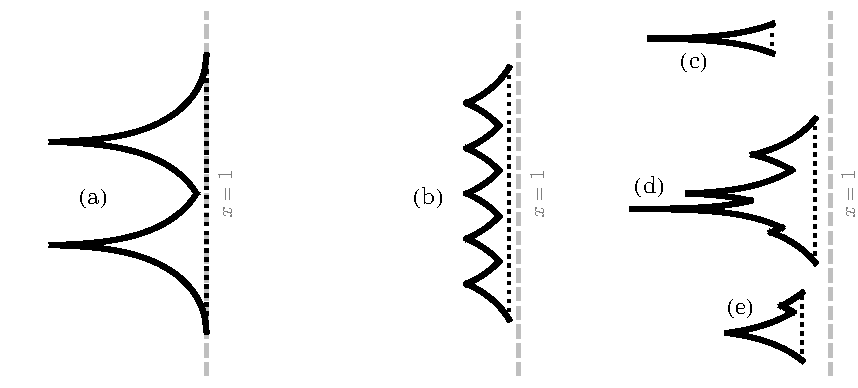
\includegraphics[width=\textwidth]{plane-domains}
  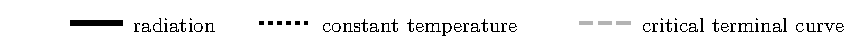
\includegraphics[width=\textwidth]{plane-domains-legend}
  \caption{
    Five domains~(a)--(e) marked out by a radiation boundary
    and a constant-temperature boundary.
    The critical terminal curve~$x = 1$ is shown for reference.
  }
  \label{fig:plane-domains}
\end{figure}

\subsection{Domain construction}
\label{sec:cartesian.plane.domain}

Since the constructed radiation boundaries only dissipate heat,
a domain for the steady conduction--radiation BVP
will not be completely specified
until there is also a boundary to supply it.
The simplest boundary condition which can supply heat
is the Dirichlet condition~$T = \const$,
and given the form of the known solution~%
  (\ref{eq:plane-scaled-laplace-solution}),
these boundaries are simply vertical lines, $x = \const$.

An infinite number of conduction--radiation domains
may therefore be marked out
by joining a constructed radiation boundary
with an appropriate Dirichlet boundary~$x = \const$,
as in Figure~\ref{fig:plane-domains}.
Each of these domains corresponds to steady conduction in the interior,
constant temperature along the right-hand side,
and thermal radiation into vacuum to the left.
Most surprising is that \emph{all} of these domains
admit the \emph{same} exact solution~(\ref{eq:plane-scaled-laplace-solution}).

Unfortunately,
the domains produced here by boundary tracing are not convex,
but \term{self-viewing}:
some of the outgoing radiation travels not to infinity,
but strikes another part of the boundary,
where it might be partially or fully absorbed.
The simple radiation boundary condition~%
  (\ref{eq:plane-scaled-radiation-boundary-condition})
is only a correct description in the absence of self-viewing radiation.
For non-convex boundaries,
modification is required to account for inbound radiation
emitted by self-viewing portions of the boundary.

\subsection{Self-viewing radiation quantified}
\label{sec:cartesian.plane.self-viewing}

It is possible to quantify the amount of self-viewing radiation,
so that we might identify instances in which it is negligible.
In Figure~\ref{fig:plane-domains} we would expect
considerable amounts of self-viewing exchange
to occur for the domains~(a), (b), (d), and~(e),
due to the adjacent spikes.
Only for a single-spike domain such as~(c)
would we expect a small amount,
so this is the case we consider here.
While the analysis thus far has been in the $xy$-plane,
the envisaged situation consists of a three-dimensional fin
whose cross section is the domain~(c).
The analysis must necessarily be conducted in three dimensions,
as radiation can be exchanged between points on the fin surface
with different~$z$.

\begin{figure}
  \savecontent{
    \centering
    \includegraphics[width=0.5\textwidth]{%
      self-viewing-radiation-elements%
    }
    \caption{
      Geometry of the area element~$\td A$
      receiving radiation from the element~$\td A^\star$.
    }
  }{fig:self-viewing-radiation-elements}
\end{figure}

Consider a differential area element~$\td A$ at the local position~%
$\positionvec = x \basisvec{x} + y \basisvec{y} + z \basisvec{z}$,
receiving radiation from a distant element~$\td A^\star$ at~%
$\positionvec^\star =
  x^\star \basisvec{x} + y^\star \basisvec{y} + z^\star \basisvec{z}$,
as shown in Figure~\ref{fig:self-viewing-radiation-elements}.
We denote the displacement from~$\positionvec^\star$ to~$\positionvec$ by
\begin{equation}
  \vec{d}^\star = \positionvec - \positionvec^\star,
  \label{eq:radiation-self-viewing-displacement}
\end{equation}
and respectively let $\theta$ and~$\theta^\star$ be the angles
that the normals~$\normalvec$ and~$\normalvec^\star$
make with this displacement.
Writing~$T$ and~$T^\star$ for the temperatures of the two elements,
the total power emitted by~$\td A^\star$
is (in scaled terms) ${T^\star}^4 \td A^\star$.
Almost none of this will strike the element~$\td A$.
Indeed it is well known~\cite{howell-2010-thermal-radiation-heat-transfer}
that the \term{view factor} from~$\td A^\star$ to~$\td A$,
defined as the fraction of radiation which leaves~$\td A^\star$
and strikes~$\td A$,
is given by
\begin{equation}
  \textq{View factor} =
    \frac{\cos\theta^\star \cos\theta \td A}{\pi {d^\star}^2},
  \label{eq:radiation-self-viewing-view-factor}
\end{equation}
where~$d^\star = \norm{\vec{d}^\star}$.
It follows that the amount of radiative power arriving at~$\td A$ is
\begin{equation}
  \textq{Power} =
    \frac{
      {T^\star}^4 \cos\theta^\star \cos\theta \td A \td A^\star
    }{
      \pi {d^\star}^2
    }.
  \label{eq:self-viewing-power}
\end{equation}
Assuming that all of this is absorbed by~$\td A$,
we see that the radiation boundary condition~%
  (\ref{eq:plane-scaled-radiation-boundary-condition})
must be modified to
\begin{equation}
  \normalvec \dotp \del T =
    -T^4 +
    \int
      \frac{
        {T^\star}^4 \cos\theta^\star \cos\theta \td A^\star
      }{
        \pi {d^\star}^2
      }
  \label{eq:plane-scaled-radiation-boundary-condition-self-viewing}
\end{equation}
in order to account for self-viewing radiation.%
\footnote{
  Since the integral term
  in~(\ref{eq:plane-scaled-radiation-boundary-condition-self-viewing})
  is \emph{non-local},
  self-viewing radiation cannot be analysed
  using the method of boundary tracing,
  which requires a local flux condition
  of the form~(\ref{eq:flux-boundary-condition}).
}
The integral is to be taken over all elements~$\td A^\star$
which can see the element~$\td A$ at the local position~$\positionvec$.
The ratio
\begin{equation}
  \savecontent{
    R =
      \frac{1}{T^4}
      \int
        \frac{
          {T^\star}^4 \cos\theta^\star \cos\theta \td A^\star
        }{
          \pi {d^\star}^2
        }
  }{eq:radiation-self-viewing-ratio}
\end{equation}
between the new integral term (for incoming radiation)
and the existing quartic term (for outgoing radiation)
provides a measure of whether self-viewing radiation is negligible
for the domains we have produced using boundary tracing.

\begin{figure}
  \savecontent{
    \centering
    \includegraphics[width=0.55\textwidth]{%
      self-viewing-radiation-elements-fin%
    }
    \caption{
      Geometry of the area elements~$\td A$ and~$\td A^\star$
      in a self-viewing concave fin
      constructed from traced boundaries on~$x_1 \le x \le x_2$.
    }
  }{fig:self-viewing-radiation-elements-fin}
\end{figure}

In the case of a single concave fin,
shaped as~$y = y (x)$ on~$x_1 \le x \le x_2$
(Figure~\ref{fig:self-viewing-radiation-elements-fin}),
it may be shown that (\ref{eq:radiation-self-viewing-ratio})~becomes
\begin{equation}
  \savecontent{
    R =
      \frac{1}{T^4}
      \int_{x_1}^{x_2}
        \smallerfrac{
          {T^\star}^4
          \squarebr[\big]{-(x - x^\star) {y'}^\star + (y - y^\star)}
          \squarebr[\big]{(x - x^\star) y' - (y - y^\star)}
          \td x^\star
        }{
          2
          \squarebr[\big]{(x - x^\star)^2 + (y - y^\star)^2}^{3/2}
          \sqrt{1 + {y'}^2}
        }
  }{eq:plane-self-viewing-ratio},
\end{equation}
where primes denote $x$-differentiation.
Details are given in Appendix~\ref{sec:self-viewing.fin}.
Numerical evaluation of this integral may be easily performed
given the expressions~(\ref{eq:plane-tracing-ode-coordinate-parametrisation-y})
and~(\ref{eq:plane-traced-boundary}) for~$y'$ and~$y$,
and the results are shown in Figure~\ref{fig:plane-self-viewing-ratio}.
While self-viewing radiation certainly cannot be neglected
if~$x_1 = 0$ or~$x_2 = 1$,
the self-viewing ratio~$R$ may be significantly reduced
by avoiding these two extremities.
There are plenty of choices which ensure that
the amount of self-viewing radiation is negligible in practice~%
($R < \SI{1}{\percent}$).
Generally speaking,
we will decrease~$R$ by shifting the chosen interval towards~$x = 0$,
although this is not surprising
given that the traced boundaries have less curvature
towards the left end (recall Figure~\ref{fig:plane-traced-boundaries}).
Alternatively we may decrease~$R$
by reducing the length~$x_2 - x_1$ of the interval
(but we note that
the temperature variation in the fin will simultaneously be reduced).

\begin{figure}
  \centredfigurecontent[width=0.55\textwidth]{plane-self-viewing-ratio}{
    Self-viewing ratio~(\ref{eq:radiation-self-viewing-ratio})
    for various fin endpoints~$(x_1, x_2)$.
    The threshold value shown is~$\SI{1}{\percent}$~\figurestyle{dotted}.
  }
\end{figure}

\subsection{Physical fin example}
\label{sec:cartesian.plane.fin}

Our analysis up to this point
has been conducted in dimensionless variables.
It is not immediately clear if our results are useful in practice,
as the temperature and length scales $\Theta$ and~$\lambda$
(i.e.~(\ref{eq:plane-temperature-scale}) and~(\ref{eq:plane-length-scale}))
depend parametrically
on both the radiation constant~$c$
and the slope~$h_0$
of the one-dimensional solution~(\ref{eq:plane-laplace-solution}).
For a given choice of material
(having emissivity~$\emiss$ and conductivity~$\conduc$),
the value of~$c$ is fixed by~(\ref{eq:radiation-constant});
only~$h_0$ can be varied freely.
To assess whether this single degree of freedom allows us to achieve
reasonable temperatures and lengths in practical applications,
we construct here an explicit physical example (in unscaled variables)
of the self-viewing fin
of Figure~\ref{fig:self-viewing-radiation-elements-fin}.
Here we restore the \scalingmarks{} which were dropped after scaling.

Suppose we want a fin
roughly $5$~times as long (in the $x$-direction)
as it is thick (in the $y$-direction).
Its half-thickness should therefore be roughly a tenth of its length.
Since
\[
  \eval*{\tder{y}{x}}_{\scaled{x}=0.55}
    = \eval*{\tder{\scaled{y}}{\scaled{x}}}_{\scaled{x}=0.55}
    = \mp 0.092
    \approx \mp 0.1,
\]
we see that the desired aspect ratio can be approximately achieved
by choosing a small $x$-interval centred on~$\scaled{x}=0.55$,
e.g.
\begin{equation}
  (\scaled{x}_1, \scaled{x}_2) = (0.5, 0.6).
  \label{eq:plane-fin-interval}
\end{equation}
In unscaled terms, the fin has length
\begin{equation}
  L = x_2 - x_1 = (\scaled{x}_2 - \scaled{x}_1) \lambda = 0.1 \lambda
  \label{eq:plane-fin-length}
\end{equation}
and thickness
\begin{equation}
  H = 2 y_2 = 2 \scaled{y}_2 \lambda = 0.0187 \lambda
  \label{eq:plane-fin-thickness}
\end{equation}
as shown in Figure~\ref{fig:plane-fin-dimensions}.%
\footnote{
  Here we ignore the issues of poor structural integrity and lethality
  associated with the pointed tip at~$x = x_1$.
}
For our choice of endpoints,
the self-viewing ratio~(\ref{eq:plane-self-viewing-ratio})
evaluates to less than~$5 \times 10^{-4}$.
Thus we may safely disregard self-viewing radiation
in the results to follow.

\begin{figure}
  \centredfigurecontent[width=0.6\textwidth]{plane-fin-dimensions}{
    Physical fin dimensions.
  }
\end{figure}

From the boundary condition~%
  (\ref{eq:plane-scaled-radiation-boundary-condition-with-groups})
(whose dimensionless group was set to unity),
we have
\begin{equation}
  \Theta
    = \roundbr*{\frac{1}{c \lambda}}^{1/3}
    = \roundbr*{\frac{\scaled{x}_2 - \scaled{x}_1}{c L}}^{1/3},
  \label{eq:plane-fin-length-scale}
\end{equation}
and therefore
\begin{equation}
  T = \scaled{T} \Theta
    = \scaled{x} \Theta
    = \scaled{x} \roundbr*{\frac{\scaled{x}_2 - \scaled{x}_1}{c L}}^{1/3}
  \label{eq:plane-fin-temperature}
\end{equation}
for the physical temperature along the fin.
Evaluating at~$\scaled{x}_2$ and~$\scaled{x}_1$
gives the temperature at the base and the tip respectively.
Figure~\ref{fig:plane-fin-temperature} shows
the corresponding Celsius temperatures%
\footnote{
  Given an absolute temperature~$T$,
  the corresponding Celsius temperature is~$t = T - \SI{273.15}{\kelvin}$,
  so that~$t / \si{\degreeCelsius} = T / \si{\kelvin} - 273.15$.
}
for an anodized aluminium fin
with emissivity~$\emiss = 0.9$~%
  \cite[Figure~4]{wade-2003-high-emissivity-aluminium-anodizing}
and conductivity~$\conduc = \SI{236}{\watt \per\metre \per\kelvin}$~%
  \cite[Figure~1]{cook-1975-thermal-electrical-conductivity-aluminium}.
For a fin of length~$L = \SI{1}{\metre}$
(and hence thickness~$H = \SI{0.19}{\metre}$),
these evaluate to $\SI{191}{\degreeCelsius}$~at the base
and $\SI{114}{\degreeCelsius}$~at the tip,
which are quite reasonable as temperatures in an engineering context.
A longer fin with a lower temperature might find application
as a heat sink on a spacecraft.
Thus boundary tracing is not merely an esoteric exercise;
highly practical results can be obtained.

\begin{figure}
  \newcommand*{\subfigurewidth}{0.48\textwidth}
  \centering
  \hspace*{\fill}
  \begin{subfigure}[t]{\subfigurewidth}
    \centredfigurecontent{plane-fin-temperature}{Celsius temperature}
  \end{subfigure}
    \hfill
  \begin{subfigure}[t]{\subfigurewidth}
    \centredfigurecontent{plane-fin-power-per-length}{Power per unit length}
  \end{subfigure}
  \hspace*{\fill}
  \caption{
    Physical quantities as a function of the fin length~$L$,
    for an anodized aluminium fin
    with scaled endpoints~(\ref{eq:plane-fin-interval}).
  }
  \label{fig:plane-fin-quantities}
\end{figure}

The physical rate of heat transfer may be estimated similarly.
The heat flux of the one-dimensional known solution is
\begin{equation}
  {-\conduc} \del T
    = -\frac{\conduc \Theta}{\lambda} \scaleddel\scaled{T}
    = -\frac{\conduc \Theta}{\lambda} \basisvec{x},
  \label{eq:plane-heat-flux}
\end{equation}
a constant vector,
representing the power dissipated in the negative $x$-direction
per unit area in the $yz$-plane.
Multiplying its magnitude by the fin thickness~$H = 2 \scaled{y}_2 \lambda$
yields
\begin{equation}
  p = 2 \scaled{y}_2 \conduc \Theta
    =
      2 \scaled{y}_2 \conduc
      \roundbr*{\frac{\scaled{x}_2 - \scaled{x}_1}{c L}}^{1/3}
  \label{eq:plane-fin-power-per-length}
\end{equation}
for the power dissipated per unit $z$-length.
The resulting curve for anodized aluminium
is displayed in Figure~\ref{fig:plane-fin-power-per-length},
and for a fin of length~$L = \SI{1}{\metre}$,
we obtain~$p = \SI{3.41}{\kilo\watt \per\metre}$.

Finally, we note that
the directional distribution of radiation emitted from a fin
will be significantly different
to that from a simple rectangular strip.
We consider the amount of radiation
arriving at a cylindrical shell (aligned with the $z$-axis)
of radius~$\rho$ (assumed large).
Following a similar analysis to the earlier self-viewing calculations,
we find that in the case of a fin
(Figure~\ref{fig:plane-directional-dependence-geometry-fin}),
the radiative power per unit area received by the cylindrical shell
is
\begin{equation}
  I =
    \frac{1}{2 \rho}
    \int_{x_1}^{x_2}
      \emiss \stefan {T^\star}^4
      ({y'}^\star \cos\varphi + \sin\varphi)
    \td x^\star,
  \label{eq:plane-directional-dependence-fin}
\end{equation}
where $\varphi$~is the angle from the negative $x$-axis.
Only a small amount of the radiative output
is sent in the $\varphi = 0$~direction
(in which the fin points),
with the majority of the radiation instead emitted laterally
(perpendicular to the two faces of the fin).
In contrast,
for a rectangular strip in the $yz$-plane
(Figure~\ref{fig:plane-directional-dependence-geometry-strip}),
we have the cosinusoidal distribution
\begin{equation}
  I = \frac{1}{2 \rho} \emiss \stefan T^4 H \cos\varphi,
  \label{eq:plane-directional-dependence-strip}
\end{equation}
where $T$~is the temperature of the strip
and $H$~is its thickness in the $y$-direction.
The normalised distributions are shown
in Figure~\ref{fig:plane-directional-dependence-fin-strip},
where the fin distribution~(\ref{eq:plane-directional-dependence-fin})
has been explicitly evaluated for our earlier fin example.
As expected,
the strip emits most of its radiative output in the direction that it faces.
This may not be desirable,
and the fin provides a useful alternative
in applications where laterally emitted radiation is preferred.

\begin{figure}
  \newcommand*{\subfigurewidth}{0.33\textwidth}
  \centering
  \hspace*{\fill}
  \begin{subfigure}[t]{\subfigurewidth}
    \centredfigurecontent{plane-directional-dependence-geometry-fin}{Fin}
  \end{subfigure}
    \hfill
  \begin{subfigure}[t]{\subfigurewidth}
    \centredfigurecontent{plane-directional-dependence-geometry-strip}{Strip}
  \end{subfigure}
  \hspace*{\fill}
  \caption{
    Directional distribution of radiative output for different shapes.
    Darker portions (along the outer ring) indicate more radiation.
  }
  \label{fig:plane-directional-dependence-geometry}
\end{figure}

\begin{figure}
  \centredfigurecontent[width=0.4\textwidth]{%
    plane-directional-dependence-fin-strip%
  }{
    Normalised directional distribution of radiative output,
    for a fin with scaled endpoints~(\ref{eq:plane-fin-interval})
    and for a rectangular strip.
  }
\end{figure}

\section{Cosinusoidal solution}
\label{sec:cartesian.cosine}

While boundary tracing as performed on
the plane-source solution~(\ref{eq:plane-laplace-solution})
did not yield convex conduction--radiation domains,
we might expect more favourable outcomes
by starting from solutions to Laplace's equation
which are not one-dimensional.
A simple class of such solutions consists of functions which are the product
of a trigonometric function in~$x$ and an hyperbolic function in~$y$.

As noted in Section~\ref{sec:cartesian.plane.domain}
we will require a boundary to supply the heat being radiated away,
and from a practical point of view it is
straight-line, constant-temperature boundaries which are of interest.
Therefore in this section we consider known solutions of the form
\begin{important}{equation}
  T = T_0 \roundbr*{1 - B \cos\frac{x}{L_0} \cosh\frac{y}{L_0}},
  \label{eq:cosine-laplace-solution}
\end{important}
where $T_0$~is a temperature scale, $L_0$~is a length scale,
and $B$~is a dimensionless constant.
The temperature is constant and takes the value~$T = T_0$
along the straight line~$x = \pi L_0/2$,
which shall ultimately serve as our heat-supplying boundary.
Physically, the constant~$B$ determines
the minimum temperature gradient along this boundary;
indeed
\begin{equation}
  \eval*{\pder{T}{x}}_{x = \pi L_0/2} = \frac{B T_0}{L_0} \cosh\frac{y}{L_0}
  \label{eq:cosine-laplace-solution-dirichlet-slope}
\end{equation}
with minimal value~$B T_0 / L_0$ at~$y = 0$,
so that solutions with a greater value of~$B$ are steeper.

\subsection{Scaling}
\label{sec:cartesian.cosine.scaling}

First we scale out the physical parameters~$T_0$ and~$L_0$.
Using the same scalings as Section~\ref{sec:cartesian.plane.scaling},
i.e.~(\ref{eq:plane-temperature-scaling}) through~(\ref{eq:plane-del-scaling}),
the radiation boundary condition~(\ref{eq:radiation-boundary-condition})
and the known solution~(\ref{eq:cosine-laplace-solution})
become
\begin{align}
  \normalvec \dotp \scaleddel \scaled{T}
    &= -\group{c \lambda \Theta^3} \scaled{T}^4,
    \label{eq:cosine-scaled-radiation-boundary-condition-with-groups}
    \\[\tallspace]
  \scaled{T}
    &=
      \group{\frac{T_0}{\Theta}}
      \roundbr*{
        1 -
          B
          \cos \roundbr*{\group{\frac{\lambda}{L_0}} \scaled{x}}
          \cosh \roundbr*{\group{\frac{\lambda}{L_0}} \scaled{y}}
      },
    \label{eq:cosine-scaled-laplace-solution-with-groups}
\end{align}
where there are two free scales, $\Theta$~(temperature) and $\lambda$~(length).
Since there are three unique dimensionless groups,
one of the groups cannot be eliminated,
and to keep the cosinusoidal terms as simple as possible
we choose the obvious scales
\begin{align}
  \Theta &= T_0,
    \label{eq:cosine-temperature-scale} \\
  \lambda &= L_0.
    \label{eq:cosine-length-scale}
\end{align}
Defining the dimensionless group
\begin{equation}
  A = \frac{1}{c L_0 {T_0}^3}
  \label{eq:cosine-dimensionless-group}
\end{equation}
and dropping \scalingmarks,
the scaled boundary condition~%
  (\ref{eq:cosine-scaled-radiation-boundary-condition-with-groups})
and known solution~(\ref{eq:cosine-scaled-laplace-solution-with-groups})
become
\begin{important}{align}
  \normalvec \dotp \del T &= -\frac{T^4}{A},
    \label{eq:cosine-scaled-radiation-boundary-condition} \\[\tallspace]
  T &= 1 - B \cos x \cosh y.
    \label{eq:cosine-scaled-laplace-solution}
\end{important}

\begin{figure}
  \centering
  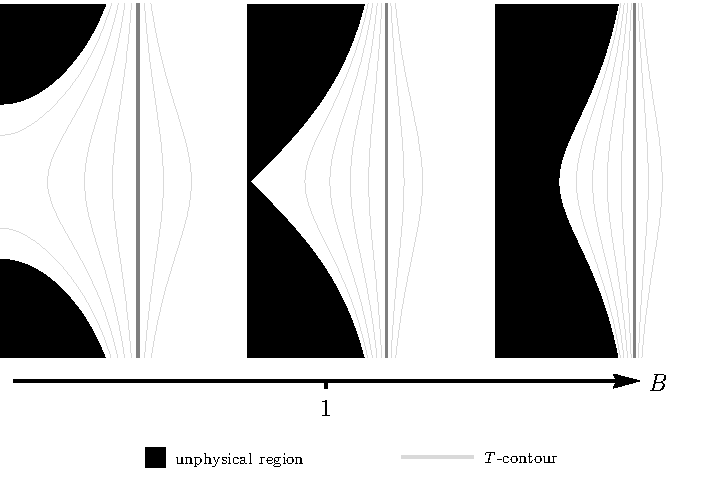
\includegraphics[width=\textwidth]{cosine-physical}
  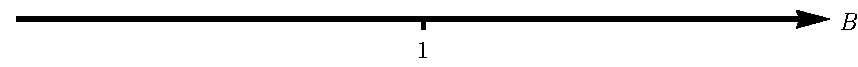
\includegraphics[width=\textwidth]{cosine-physical-arrow}
  
\includegraphics[width=\textwidth]{cosine-physical-legend}
  \caption{
    Unphysical region~$T < 0$
    for the known solution~(\ref{eq:cosine-scaled-laplace-solution}),
    as $B$~increases.
    In each plot, the left edge is~$x = 0$
    and the thick grey vertical line is~$x = \pi/2$,
    which is also the contour~$T = 1$.
  }
  \label{fig:cosine-physical}
\end{figure}

\subsection{Physical region}
\label{sec:cartesian.cosine.physical}

Since it is the straight-line boundary~$x = \pi/2$
which ultimately shall, in the form of a Dirichlet condition~$T = 1$,
supply the heat to be conducted and radiated away,
only the side on which~$T \le 1$ is relevant,
namely the side~$x \le \pi/2$.
Given that the known solution~(\ref{eq:cosine-scaled-laplace-solution})
is an even function of~$x$,
it also suffices to consider~$x \ge 0$ only.

Thus the region of interest
is the vertical strip~$0 \le x \le \pi/2$.
Not all of this strip is physically relevant
as only positive temperatures are admissible
in thermal radiation problems.
Since the known solution~(\ref{eq:cosine-scaled-laplace-solution})
vanishes along~$\cos x \cosh y = 1 / B$,
the geometry of the physical region~$T \ge 0$
will depend on the value of the dimensionless constant~$B$
(see Figure~\ref{fig:cosine-physical}).
The unphysical region~$T < 0$ is omitted from the remainder of the analysis,
as physically meaningful radiation boundaries cannot be found there.

\subsection{Boundary tracing equations}
\label{sec:cartesian.cosine.tracing}

In addition to only considering the physical region~$T \ge 0$,
traced boundaries will only exist within the viable domain~$\Phi \ge 0$.
For the boundary condition~%
  (\ref{eq:cosine-scaled-radiation-boundary-condition})
and known solution~(\ref{eq:cosine-scaled-laplace-solution}) at hand,
we obtain the derivatives
\begin{align}
  P &= \pder{T}{x} = +B \sin x \cosh y,
    \label{eq:cosine-gradient-x-component} \\[\tallspace]
  Q &= \pder{T}{y} = -B \cos x \sinh y,
    \label{eq:cosine-gradient-y-component}
\end{align}
the flux function
\begin{equation}
  F = -\frac{(1 - B \cos x \cosh y) ^ 4}{A},
  \label{eq:cosine-flux-function}
\end{equation}
and the viability function
\begin{align*}
  \Phi
  &= (\del T)^2 - F^2 \\
  &=
    B^2 \roundbr*{\sin^2 x + \sinh^2 y}
      -
    \frac{(1 - B \cos x \cosh y) ^ 8}{A^2}.
    \yesnumber
    \label{eq:cosine-viability-function}
\end{align*}
The geometry of the viable domain~$\Phi \ge 0$
therefore depends on both of the dimensionless parameters~$A$ and~$B$,
as does the boundary tracing ODE~%
  (\ref{eq:tracing-ode-coordinate-parametrisation-u}),
which becomes
\begin{important}{equation}
  \tder{x}{y} = \frac{P Q \mp F \sqrt{\Phi}}{Q^2 - F^2}.
  \label{eq:cosine-tracing-ode-coordinate-parametrisation-x}
\end{important}
Given the complexity of managing more than one parameter,
we consider~$B = 1$ before examining the general case.

\subsection{Simple case (\texorpdfstring{$B = 1$}{B = 1})}
\label{sec:cartesian.cosine.simple}

\subsubsection{Viable domain}
\label{sec:cartesian.cosine.simple.viable}

In the $B = 1$~case,
the known solution~(\ref{eq:cosine-scaled-laplace-solution}) simplifies to
\begin{equation}
  T = 1 - \cos x \cosh y
  \label{eq:cosine-simple-laplace-solution}
\end{equation}
and the viability function~(\ref{eq:cosine-viability-function}) reduces to
\begin{equation}
  \Phi = \sin^2 x + \sinh^2 y - \frac{(1 - \cos x \cosh y) ^ 8}{A^2}.
  \label{eq:cosine-simple-viability-function}
\end{equation}
The dependence of the non-viable domain~$\Phi < 0$
on the dimensionless group~$A$
is shown in Figure~\ref{fig:cosine_simple-physical-viable}.
Radiation boundaries as produced by boundary tracing
will only be found in the white region,
which is both physical~($T \ge 0$) and viable~($\Phi \ge 0$).

The non-viable domain consists of a single%
\footnote{
  There also exist non-viable regions
  (not shown in Figure~\ref{fig:cosine_simple-physical-viable})
  which lie within the unphysical region~$T < 0$,
  but we recall that the unphysical region has been omitted from the analysis
  due to physical irrelevance.
}
non-viable region which recedes towards the right as $A$~increases.
Not obvious from Figure~\ref{fig:cosine_simple-physical-viable} however
is that the boundary of this single non-viable region,
henceforth called the \term{proper} terminal curve,
only constitutes \emph{almost all} of the terminal curve.
The full terminal curve consists of the proper terminal curve
together with the origin~$(x, y) = (0, 0)$,
which is a terminal point
by virtue of being an isolated root of the equation~$\Phi = 0$.

\begin{figure}
  \centering
  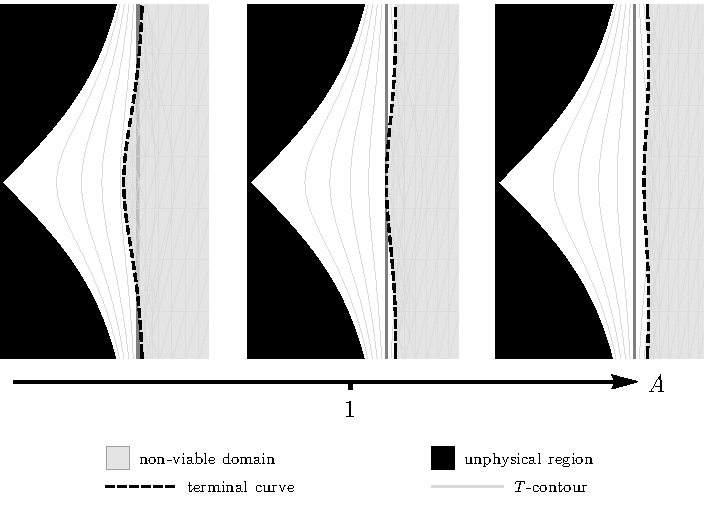
\includegraphics[width=\textwidth]{cosine_simple-physical-viable}
  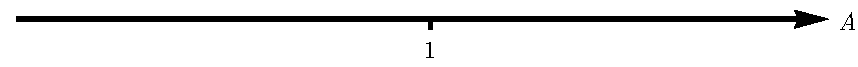
\includegraphics[width=\textwidth]{cosine_simple-physical-viable-arrow}
  
\includegraphics[width=\textwidth]{cosine_simple-physical-viable-legend}
  \caption{
    Non-viable domain~$\Phi < 0$
    for the known solution~(\ref{eq:cosine-simple-laplace-solution})
    and viability function~(\ref{eq:cosine-simple-viability-function}),
    as $A$~increases.
    In each plot, the left edge is~$x = 0$
    and the thick grey vertical line is~$x = \pi/2$,
    which is also the contour~$T = 1$.
  }
  \label{fig:cosine_simple-physical-viable}
\end{figure}

\subsubsection{Boundary tracing}
\label{sec:cartesian.cosine.simple.tracing}

The tracing ODE~%
  (\ref{eq:cosine-tracing-ode-coordinate-parametrisation-x})
cannot be integrated analytically,
so the traced boundaries are determined numerically.
In doing so, the parametrisation~$x = x (y)$
is unable to handle traced boundaries which are locally horizontal;
such difficulty is avoided by instead using the arc-length parametrisation~%
  (\ref{eq:tracing-ode-arc-length-parametrisation-u})
\&~(\ref{eq:tracing-ode-arc-length-parametrisation-v}),
which for Cartesian coordinates reduces to
\begin{align}
  \tder{x}{s} &= \frac{-Q F \pm P \sqrt{\Phi}}{(\del T)^2},
    \label{eq:cosine-tracing-ode-arc-length-parametrisation-x} \\[\tallspace]
  \tder{y}{s} &= \frac{+P F \pm Q \sqrt{\Phi}}{(\del T)^2}.
    \label{eq:cosine-tracing-ode-arc-length-parametrisation-y}
\end{align}
Two branches of traced boundaries are obtained
by integrating forward
from starting points within the region
both physical~($T \ge 0$) and viable~($\Phi \ge 0$).
The resulting curves (Figure~\ref{fig:cosine_simple-traced-boundaries})
are boundaries along which the radiation boundary condition~%
  (\ref{eq:cosine-scaled-radiation-boundary-condition})
is satisfied.
For the correct boundary orientation,
note that the temperature~$T$ is an increasing function of~$x$;
it follows that the interior lies to the right of each boundary curve,
with heat being lost by radiation to the left.

\begin{figure}
  \centredfigurecontent[width=0.42\textwidth]{%
    cosine_simple-traced-boundaries%
  }{
    Traced boundaries for~$A = 0.5$,
    obtained by integrating
    (\ref{eq:cosine-tracing-ode-arc-length-parametrisation-x})
    \&~(\ref{eq:cosine-tracing-ode-arc-length-parametrisation-y}).
  }
\end{figure}

By patching together the traced boundaries,
an unlimited number of radiation boundaries may be constructed.
However, almost all such constructions are non-convex
(see Figure~\ref{fig:cosine_simple-traced-boundaries-patched-spiky}).
At any point \emph{strictly} within the viable domain,
i.e.~$\Phi > 0$,
the two traced boundaries through it will cross at a non-zero angle,
and patching these two boundaries together
inevitably results in a spike made of non-convex curves.
As noted already in Section~\ref{sec:cartesian.plane.domain},
self-viewing radiation is not accounted for
by the simple radiation boundary condition~%
  (\ref{eq:cosine-scaled-radiation-boundary-condition}),
and so the non-convex constructions are all invalid.

\begin{figure}
  \newcommand*{\subfigurewidth}{0.36\textwidth}
  \centering
  \hspace*{\fill}
  \begin{subfigure}[t]{\subfigurewidth}
    \centredfigurecontent{cosine_simple-traced-boundaries-patched-spiky}{%
      Spiky non-convex boundary
    }
  \end{subfigure}
    \hfill
  \begin{subfigure}[t]{\subfigurewidth}
    \centredfigurecontent{cosine_simple-traced-boundaries-patched-smooth}{%
      Smooth candidate boundary
    }
  \end{subfigure}
  \hspace*{\fill}
  \caption{
    Radiation boundaries~\figurestyle{thick black} patched together
    using traced boundaries~\figurestyle{grey}.
  }
  \label{fig:cosine_simple-traced-boundaries-patched}
\end{figure}

\begin{figure}
  \centredfigurecontent[width=0.63\textwidth]{%
    cosine_simple-terminal-points%
  }{
    $T$-contours which intersect the proper terminal curve~$\Phi = 0$,
    which is the border of the non-viable domain~$\Phi < 0$.
    The horizontal scale is exaggerated.
  }
\end{figure}

To avoid the non-convex spikes,
the join must occur at a point along the terminal curve~$\Phi = 0$.
Specifically this point must not be an ordinary terminal point,
at which the two traced boundaries being patched
would form a cusp with inconsistent boundary orientation
(see Section~\ref{sec:introduction.tracing}).
Instead the join must occur at a critical terminal point;
we recall that this is a point along the terminal curve
for which the local $T$-contour touches the terminal curve~$\Phi = 0$
tangentially (rather than crossing at a non-zero angle).

Now in the present situation,
the full terminal curve consists of
an isolated terminal point at the origin
in union with the proper terminal curve
(which is the boundary of the non-viable region
visible in Figure~\ref{fig:cosine_simple-physical-viable}).
The terminal point at the origin is already notable due to its isolation,
but even more remarkable is that the local $T$-contour~($T = 0$)
looks like~$y = \pm x$.
One therefore wonders:
  are the local $T$-contour (whose tangent is indeterminate)
  and the local portion of the terminal curve (which is just a point)
  \emph{tangential}, and therefore,
  is the origin a \emph{critical} terminal point?
While the tangency is debatable,
the answer to the criticality question ought to be yes
on account of the actual behaviour:
two traced boundaries pass through the origin
(see Figure~\ref{fig:cosine_simple-traced-boundaries})
as if it were an hyperbolic critical terminal point,
with $y = 0$~as the common tangent.
Unfortunately the pair of traced boundaries forms a non-convex spike,
which is of no use here.

With the origin ruled out,
it remains to consider the proper terminal curve.
Figure~\ref{fig:cosine_simple-terminal-points} shows that in the present case,
all points along the proper terminal curve are ordinary
except for a single critical terminal point~$(x, y) = (x_0, 0)$
at the intersection of the proper terminal curve
and the horizontal axis~$y = 0$.
Algebraically, $x_0$~is the positive%
\footnote{
  The trivial solution~$x = 0$
  corresponds to the isolated terminal point at the origin,
  which we have just dismissed.
}
solution to
\begin{equation}
  \eval[\textsize]{\Phi}_{y=0}
  = \roundbr*{1 - \cos^2 x} - \frac{(1 - \cos x)^8}{A^2}
  = 0,
  \label{eq:cosine-simple-critical-terminal-point-x}
\end{equation}
a polynomial equation in~$\cos x$.
Furthermore, the local $T$-contour through~$(x_0, 0)$
lies on the viable side of the proper terminal curve;
therefore the critical terminal point~$(x_0, 0)$ is of hyperbolic type,
with two traced boundaries passing through it smoothly.
By patching together the portions of traced boundary
which lie to the right of~$(x_0, 0)$,
a single spike-free radiation boundary can be constructed
as shown in Figure~\ref{fig:cosine_simple-traced-boundaries-patched-smooth};
this boundary shall be referred to as the \term{candidate boundary}.
It is interesting to note that
the candidate boundary and the proper terminal curve
are virtually indistinguishable,
despite only touching each other at the critical terminal point~$(x_0, 0)$.

\subsubsection{Convexity}
\label{sec:cartesian.cosine.simple.convexity}

The choice of the candidate boundary over all other boundary patchings
is a necessary but not sufficient condition for convexity.
While the candidate boundary is convex at~$(x_0, 0)$,
it will eventually inflect
at some~$(x, y) = (x_\infl, \pm y_\infl)$ depending on~$A$,
and become concave.

Recalling the goal of constructing domains
corresponding to a conduction--radiation BVP\@,
a \term{candidate domain} is demarcated by using
the candidate boundary as the radiation boundary
and the straight line~$x = \pi/2$
as a constant-temperature heat-supplying boundary.
The continuum of candidate domains (for~$0 < A < 1$)\footnote{
  At~$A = 1$ the candidate boundary touches the line~$x = \pi/2$,
  and the candidate domain shrinks to a point.
}
is shown in Figure~\ref{fig:cosine_simple-candidate-domains};
each domain is shaped like a thin lens,
corresponding to steady conduction in its interior,
thermal radiation along the curved boundary to the left,
and constant temperature~$T = 1$ along the straight boundary on the right.
The domain will be valid if the curved boundary
(which is a portion of the corresponding candidate boundary)
is convex, or equivalently,
if the first inflection of the corresponding candidate boundary
occurs at abscissa~$x_\infl \ge \pi/2$.

\begin{figure}
  \newcommand*{\legendtrimwidth}{0.1\textwidth}
  \newcommand*{\legendoffsetheight}{0.36\textwidth}
  \centering
  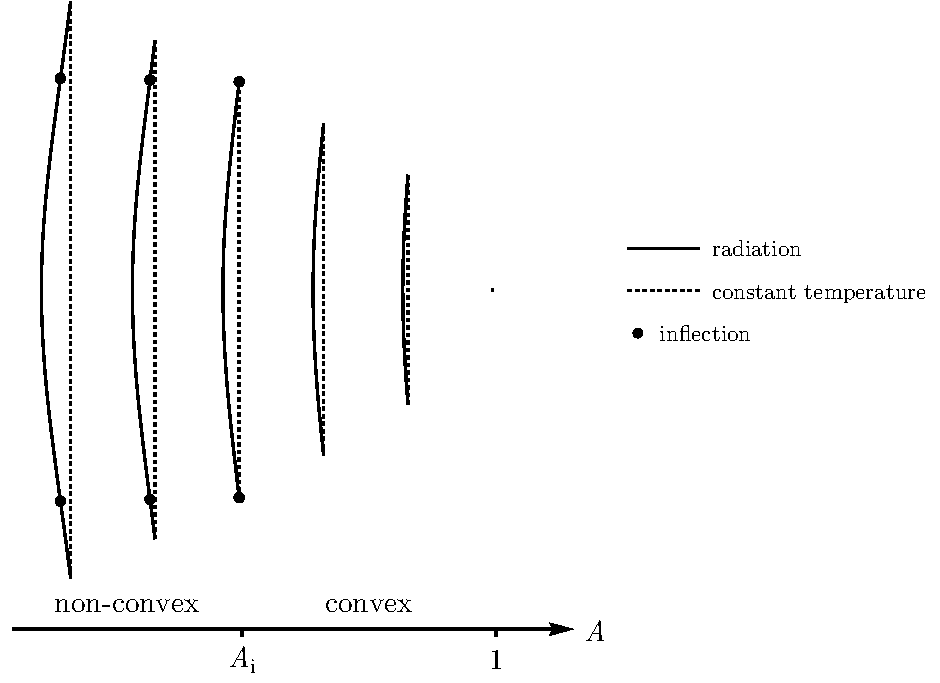
\includegraphics[width=0.6\textwidth]{cosine_simple-candidate-domains}
  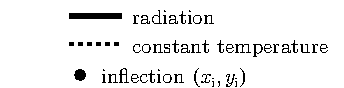
\includegraphics[
    width={0.4\textwidth-\legendtrimwidth},
    trim={\legendtrimwidth} {-\legendoffsetheight} 0 0,
  ]{cosine_simple-candidate-domains-legend}
  \caption{
    Candidate domains marked out by a radiation boundary
    and the constant-temperature boundary~$x = \pi/2$,
    as $A$~increases.
    Points of inflection are shown for reference.
  }
  \label{fig:cosine_simple-candidate-domains}
\end{figure}

The critical value~$A = A_\infl$
(where the candidate domain changes from invalid to valid)
is that for which the first inflection occurs at precisely~$x_\infl = \pi/2$.
Given that the candidate boundary is never horizontal,
$A_\infl$~is best sought using the coordinate parametrisation~$x = x (y)$
for the candidate boundary.
In Cartesian coordinates, points of inflection
are simply given by zero-crossings in the second derivative,
or, using primes for $y$-differentiation, $x''$.
Differentiating the first derivative~%
  (\ref{eq:cosine-tracing-ode-coordinate-parametrisation-x})
gives
\begin{equation}
  x'' = \tder{}{y} \roundbr*{\frac{P Q \mp F \sqrt{\Phi}}{Q^2 - F^2}},
  \label{eq:acceleration-traced-boundary-cartesian-by-y}
\end{equation}
whose right-hand side may be reduced to a function purely of~$x$ and~$y$
by using~(\ref{eq:cosine-tracing-ode-coordinate-parametrisation-x})
to eliminate the first derivatives.
Substituting~$x = x_\infl = \pi/2$, this becomes
\begin{equation}
  \eval[\textsize]{x''}_{x=\pi/2} =
    \frac{A^2 C}{\sqrt{A^2 C^2 - 1}}
    \squarebr*{
      2 S - \roundbr*{1 + S^2} \roundbr*{A^2 S + 4 \sqrt{A^2 (1 + S^2) - 1}}
    },
  \label{eq:%
    cosine-simple-traced-boundary-acceleration-cartesian-by-y-inflection%
  }
\end{equation}
where $C = \cosh y$ and~$S = \sinh y$.
Only the square-bracketed factor can change sign,
and an analysis shows that for~$0 < A < 1$,
this factor has a unique zero-crossing~$S = S_\infl (A)$.
The would-be $y$-coordinate of inflection for a given~$A$ is therefore
\begin{equation}
  y = y_\infl (A) = \sinh^{-1} \roundbr[\bulkysize]{S_\infl (A)}.
  \label{eq:cosine-simple-traced-boundary-y-would-be-inflection}
\end{equation}
Since the inflection is supposed to occur at~$x_\infl = \pi/2$,
the critical value~$A = A_\infl$ is the solution to
\begin{equation}
  x \roundbr[\bulkysize]{y_\infl (A)} = \pi/2,
  \label{eq:cosine-simple-traced-boundary-a-inflection-equation}
\end{equation}
whose left-hand side is the coordinate parametrisation~$x = x (y)$
evaluated at the would-be $y$-coordinate~%
  (\ref{eq:cosine-simple-traced-boundary-y-would-be-inflection}).
Using the bisection algorithm we obtain the root
\begin{equation}
  A_\infl = 0.79718.
  \label{eq:cosine-simple-traced-boundary-a-inflection}
\end{equation}
Therefore, the lens-like candidate domain for a given~$A$ is convex
if and only if
\begin{equation}
  A_\infl \le A < 1.
  \label{eq:cosine-simple-traced-boundary-convex-a-interval}
\end{equation}

\subsubsection{Near-convex self-viewing radiation}
\label{sec:cartesian.cosine.simple.self-viewing}

While the candidate domains for~$0 < A < A_\infl$ are not convex,
one would expect the amount of self-viewing radiation to be small
in cases where $A$~is not significantly less than~$A_\infl$.
In the same vein as Section~\ref{sec:cartesian.plane.self-viewing},
we may obtain an explicit integral expression
for the ratio~(\ref{eq:radiation-self-viewing-ratio}),
which quantifies the amount of self-viewing radiation
that has been neglected.

\begin{figure}
  \newcommand*{\subfigurewidth}{0.325\textwidth}
  \centering
  \begin{subfigure}{\subfigurewidth}
    \centredfigurecontent{cosine_simple-self-viewing-bounds-none}{
      $y < y_\view$
    }
  \end{subfigure}
  \hfill
  \begin{subfigure}{\subfigurewidth}
    \centredfigurecontent{cosine_simple-self-viewing-bounds-concave}{
      $y_\view < y < y_\infl$
    }
  \end{subfigure}
  \hfill
  \begin{subfigure}{\subfigurewidth}
    \centredfigurecontent{cosine_simple-self-viewing-bounds-both}{
      $y_\infl < y < y_\End$
    }
  \end{subfigure}
  \caption{
    Portion~$y_1 \le y^\star \le y_2$~\figurestyle{grey}
    of a candidate boundary
    which imparts self-viewing radiation onto the point~%
    $\positionvec = x \basisvec{x} + y \basisvec{y}$~\figurestyle{X-mark}.
    No radiation is imparted
    in case~(\subref*{fig:cosine_simple-self-viewing-bounds-none}).
  }
  \label{fig:cosine_simple-self-viewing-bounds}
\end{figure}

By symmetry
we need only consider the top half~$y > 0$ of each candidate domain,
and after a similar analysis to Appendix~\ref{sec:self-viewing.fin},
we obtain
\begin{equation}
  \savecontent{
    R =
      \frac{1}{T^4}
      \int_{y_1}^{y_2}
        \smallerfrac{
          {T^\star}^4
          \squarebr[\big]{-(x - x^\star) + (y - y^\star) {x'}^\star}
          \squarebr[\big]{(x - x^\star) - (y - y^\star) x'}
          \td y^\star
        }{
          2
          \squarebr[\big]{(x - x^\star)^2 + (y - y^\star)^2}^{3/2}
          \sqrt{{x'}^2 + 1}
        }
  }{eq:cosine-simple-self-viewing-ratio},
\end{equation}
where $y_1 \le y^\star \le y_2$~is the interval of
all elements that can impart radiation
onto the local element at~$\positionvec = x \basisvec{x} + y \basisvec{y}$.
The geometry of the candidate domains is such that
$y_1$ and~$y_2$ depend non-trivially upon~$\positionvec$.
We write~$(x, y) = (\pi/2, y_\End)$ for the uppermost tip,
and let $(x_\view, y_\view)$~be the lowest point on the radiation boundary
that is visible from~$(\pi/2, y_\End)$.
From Figure~\ref{fig:cosine_simple-self-viewing-bounds},
we see that self-viewing radiation is received either
(\subref*{fig:cosine_simple-self-viewing-bounds-none})~%
  not at all,
(\subref*{fig:cosine_simple-self-viewing-bounds-concave})~%
  from part of the concave portion, or
(\subref*{fig:cosine_simple-self-viewing-bounds-both})~%
  from all of the concave portion and part of the convex portion,
depending on the location of the receiving point~$\positionvec$
in relation to both the lowest self-viewing point~$(x_\view, y_\view)$
and the point of inflection~$(x_\infl, y_\infl)$.

\begin{figure}
  \centredfigurecontent[width=0.52\textwidth]{%
    cosine_simple-self-viewing-ratio-bound%
  }{
    Upper bound~(\ref{eq:cosine-simple-self-viewing-ratio-bound})
    for the self-viewing ratio in a candidate domain.
  }
\end{figure}

We would like to determine an interval~$A_\prac \le A < A_\infl$
in which the amount of self-viewing radiation is practically negligible,
despite the candidate domain being non-convex.
In this regard,
there are two difficulties
with the integral expression~(\ref{eq:cosine-simple-self-viewing-ratio}).
Firstly, as noted above,
the bounds~$y_1$ and~$y_2$ depend on the local position~$(x, y)$;
secondly, the result of the integration is a function of~$y$
(on the interval~$y_\view \le y \le y_\End$
where self-viewing radiation is possible).
The simplest way forward is to determine
an upper bound for~(\ref{eq:cosine-simple-self-viewing-ratio}),
so that for each given value of~$A$
we may obtain a single $R$-value rather than a function of~$y$.
The analysis of Appendix~\ref{sec:self-viewing.lens} yields
\begin{equation}
  \savecontent{
    R \le R_+ =
      \frac{
        (T_{\max} / T_{\min})^4
        \abs{x''}_{\max}^2
        (y_\End - y_\view)^2
      }{
        8 \roundbr*{\abs{x'}_{\min}^2 + 1}^2
      }
  }{eq:cosine-simple-self-viewing-ratio-bound},
\end{equation}
and from Figure~\ref{fig:cosine_simple-self-viewing-ratio-bound}
we see that the upper bound~$R_+$ falls below~$\SI{1}{\percent}$ at
\begin{equation}
  A = A_\prac = 0.43124.
  \label{eq:cosine-simple-traced-boundary-a-practical}
\end{equation}
Therefore, while exactness cannot be claimed for any candidate domain
in the continuum~$0 < A < A_\infl$ of non-convexity,
self-viewing radiation may be ignored to good approximation
on the interval
\begin{equation}
  A_\prac \le A < A_\infl.
  \label{eq:cosine-simple-traced-boundary-practical-a-interval}
\end{equation}
Thus we extend the range of practically useful results
beyond the interval~(\ref{eq:cosine-simple-traced-boundary-convex-a-interval})
of convexity.

\subsection{General case (\texorpdfstring{$B$~arbitrary}{B arbitrary})}
\label{sec:cartesian.cosine.general}

\subsubsection{Viable domain}
\label{sec:cartesian.cosine.general.viable}

In the general case the dimensionless group~$B$ may also be varied,
and altogether the parameter space~$(A, B)$ is two-dimensional.
Two degrees of freedom is too many to manage,
and the behaviour of the viable domain is best understood
by fixing~$A$ and varying~$B$.

\begin{figure}
  \newcommand*{\legendoffsetheight}{0.1\textwidth}
  \centering
  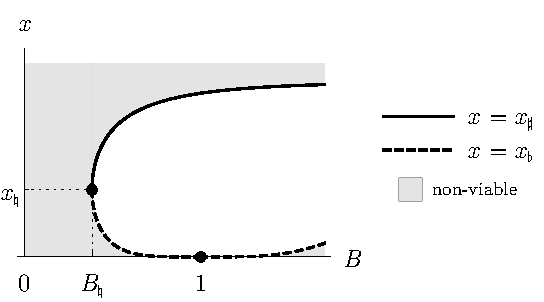
\includegraphics[width=0.45\textwidth]{cosine_general-critical}
  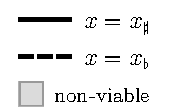
\includegraphics[
    width=0.2\textwidth,
    trim=0 {-\legendoffsetheight} 0 0,
  ]{cosine_general-critical-legend}
  \caption{
    Terminal points along the $x$-axis, as $B$~increases with $A$~fixed.
  }
  \label{fig:cosine_general-critical}
\end{figure}

Of particular interest are the terminal points along the $x$-axis;
these are necessarily critical terminal points
because the local $T$-contour and the terminal curve~$\Phi = 0$
both cross the $x$-axis vertically
(as $T$ and~$\Phi$ are both even functions of~$y$),
and are therefore tangential.
Algebraically these terminal points are given by the roots of
\begin{equation}
  \eval[\textsize]{\Phi}_{y=0}
  = B^2 \sin^2 x - \frac{(1 - B \cos x)^8}{A^2}
  = 0,
  \label{eq:cosine-general-critical-terminal-point-x}
\end{equation}
which are shown in Figure~\ref{fig:cosine_general-critical}.
For sufficiently small~$B$,
there are no roots and the entire $x$-axis is non-viable,
until a single root~$x = x_\nat (A)$ appears at~$B = B_\nat (A)$.
As $B$~increases past this transitional value,
the root splits into two roots, $x = x_\flat (A, B)$ and~$x = x_\sharp (A, B)$.
At~$B = 1$, the lesser root~$x_\flat$ vanishes,
before becoming positive again.
In terms of the viable domain, this translates into five cases
(Figure~\ref{fig:cosine_general-physical-viable}):
\begin{enumerate}
  \item
    \label{itm:cartesian.cosine.general.cases.gentle}
    \term{Gentle regime}, $B < B_\nat (A)$:
    The non-viable domain completely envelopes the $x$-axis,
    dividing the viable domain into two halves.
    Two hyperbolic critical terminal points exist along the $y$-axis
    at~$(x, y) = (0, \pm y_0)$.
  \item
    \label{itm:cartesian.cosine.general.cases.gentle-to-fair}
    \term{Gentle-to-fair transition}, $B = B_\nat (A)$:
    The two viable regions pinch together at~$(x, y) = (x_\nat, 0)$,
    a critical terminal point of hyperbolic type.%
    \footnote{
      Here the local $T$-contour crosses the $x$-axis vertically
      while the terminal curve~$\Phi = 0$ has indeterminate tangent
      (being the location of a self-intersection).
      While the tangency is again debatable,
      two traced boundaries pass through vertically
      as if the vertical line~$x = x_\nat$ were the common tangent.
    }
    The non-viable domain now consists of two disjoint regions.
  \item
    \label{itm:cartesian.cosine.general.cases.fair}
    \term{Fair regime}, $B_\nat (A) < B < 1$:
    The two non-viable regions are sundered further apart
    by a growing viable tract along the $x$-axis,
    with $(x_\nat, 0)$~splitting into the two
    hyperbolic critical terminal points~$(x_\flat, 0)$ and~$(x_\sharp, 0)$.
  \item
    \label{itm:cartesian.cosine.general.cases.fair-to-steep}
    \term{Fair-to-steep transition}, $B = 1$:
    This is the simple case
    of Section~\ref{sec:cartesian.cosine.simple};
    the hyperbolic critical terminal point~$(x_\sharp, 0)$
    is what was formerly called~$(x_0, 0)$.
    The smaller non-viable region of the fair regime
    has shrunken to nothingness,
    and the critical terminal points~$(0, \pm y_0)$ and~$(x_\flat, 0)$
    have merged together
    to form the isolated critical terminal point at the origin.
  \item
    \label{itm:cartesian.cosine.general.cases.steep}
    \term{Steep regime}, $B > 1$:
    The smaller non-viable region
    reappears but is overrun by the growing unphysical region.
    The critical terminal points~$(0, \pm y_0)$ (if they exist)
    and~$(x_\flat, 0)$ all lie in the unphysical region
    and are therefore irrelevant,
    leaving a single hyperbolic critical terminal point~$(x_\sharp, 0)$.
\end{enumerate}

\subsubsection{Boundary tracing}
\label{sec:cartesian.cosine.general.tracing}

An exhaustive treatment cannot be given here
due to the complex dependence
of the known solution~$T$ and the viability function~$\Phi$
on both~$A$ and~$B$.
Nevertheless, broad statements can be made.

\begin{figure}
  \centering
  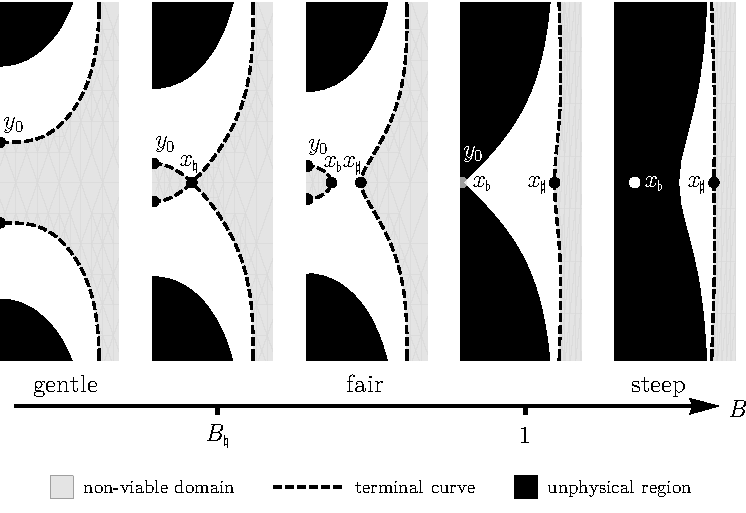
\includegraphics[width=\textwidth]{cosine_general-physical-viable}
  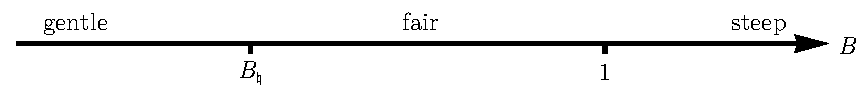
\includegraphics[width=\textwidth]{cosine_general-physical-viable-arrow}
  
\includegraphics[width=\textwidth]{cosine_general-physical-viable-legend}
  \caption{
    Non-viable domain~$\Phi < 0$ and critical terminal points
    for the known solution~(\ref{eq:cosine-scaled-laplace-solution})
    and viability function~(\ref{eq:cosine-viability-function}),
    as $B$~increases with $A$~fixed.
    In each plot, the left edge is~$x = 0$ and the right edge is~$x = 2$.
  }
  \label{fig:cosine_general-physical-viable}
\end{figure}

In Case~\ref{itm:cartesian.cosine.general.cases.gentle} (gentle regime)
only non-convex spikes can be formed
by patching together traced boundaries,
even at the critical terminal points~$(0, \pm y_0)$ along the $y$-axis.
Case~\ref{itm:cartesian.cosine.general.cases.fair-to-steep}
  (fair-to-steep transition)
is the simple $B = 1$~case which we have already analysed
in Section~\ref{sec:cartesian.cosine.simple};
recall that a conduction--radiation domain in the shape of a convex lens
can be produced for each~$A$ in the interval~%
  (\ref{eq:cosine-simple-traced-boundary-convex-a-interval})
by using the traced boundaries which pass through~$(x_0, 0)$
(now called~$(x_\sharp, 0)$).
The situation in
Case~\ref{itm:cartesian.cosine.general.cases.steep} (steep regime)
is very similar,
but the convex lens shapes which can be produced
are even thinner than those of
Case~\ref{itm:cartesian.cosine.general.cases.fair-to-steep}.

This leaves
Case~\ref{itm:cartesian.cosine.general.cases.gentle-to-fair}
  (gentle-to-fair transition)
and
Case~\ref{itm:cartesian.cosine.general.cases.fair} (fair regime),
the former of which need not be treated separately
since it is effectively a degenerate version of the latter
(with~$x_\flat = x_\sharp$).
In the same manner as a spike-free candidate boundary
was constructed through~$(x_0, 0)$
in Section~\ref{sec:cartesian.cosine.general.viable},
so may candidate boundaries be constructed
through the hyperbolic critical terminal points~%
  $(x_\flat, 0)$ and~$(x_\sharp, 0)$.
Again we can form lens-shaped candidate domains,
and these will be convex for sufficiently well-chosen~$A$ and~$B$.

Much more interesting however is the existence
in Case~\ref{itm:cartesian.cosine.general.cases.fair} (fair regime)
of convex conduction--radiation domains
which are \emph{not} shaped as lenses.
We cannot perform a general analysis here
due to the complex dependence of the curvature on~$A$ and~$B$,
so we look at the illustrative example~$(A, B) = (12, 0.082506)$.
Figure~\ref{fig:cosine_general-traced-boundaries-convex}
shows (among other features) the frontiers of inflection
for the two branches of traced boundaries,
which we obtain by computing the zero-contours of the second derivative~%
  (\ref{eq:acceleration-traced-boundary-cartesian-by-y})
using numerical integration.
Only the portions of traced boundary which lie
convex side of the inflection frontiers
will be valid as radiation boundaries.
Since the end is to construct a domain
with the straight line contour~$x = \pi/2$
serving as the constant-temperature boundary,
we immediately discard any convex portion of traced boundary
which does not reach~$x = \pi/2$.
Of the remaining convex portions,
those which do not reach the $x$-axis~($y = 0$)
are unable to join up with a convex portion of the opposite branch
(which is necessary to form a complete domain boundary);
discarding those also leaves the convex portions of traced boundary
shown in Figure~\ref{fig:cosine_general-traced-boundaries-convex}.

\begin{figure}
  \newcommand*{\subfigurewidth}{0.45\textwidth}
  \centering
  \includegraphics[width=\textwidth, trim=0 -10 0 0]%
    {cosine_general-asymmetric-construction-legend}
  \hspace*{\fill}
  \begin{subfigure}[t]{\subfigurewidth}
    \centredfigurecontent{cosine_general-traced-boundaries-convex}{%
      Convex portions of the two branches of traced boundaries
      which reach both the constant-temperature boundary~$x = \pi/2$
      and the $x$-axis.
    }
  \end{subfigure}
  \hfill
  \begin{subfigure}[t]{\subfigurewidth}
    \centredfigurecontent{cosine_general-asymmetric_domain}{%
      An asymmetric domain marked out by a radiation boundary
      and the constant-temperature boundary~$x = \pi/2$.
    }
  \end{subfigure}
  \hspace*{\fill}
  \caption{
    Constructing an asymmetric conduction--radiation domain
    for~$(A, B) = (12, 0.082506)$ (fair regime).
  }
  \label{fig:cosine_general-asymmetric-construction}
\end{figure}

The smooth traced boundary through the critical terminal point~$(x_\sharp, 0)$
may be used to construct the familiar lens-shaped domain.
The remaining convex portions of traced boundary
shown in Figure~\ref{fig:cosine_general-traced-boundaries-convex}
can be used to construct conduction--radiation domains
which are not lens-shaped, including asymmetric domains
(Figure~\ref{fig:cosine_general-asymmetric_domain});
simply take two intersecting traced boundaries
(one from the lower branch and one from the upper)
which are not reflections of each other,
and trim them at their intersection
and where they meet the constant-temperature boundary~$x = \pi/2$.
It is most remarkable that
\emph{any} conduction--radiation domain constructed in this manner
will admit the very same exact solution~%
  (\ref{eq:cosine-scaled-laplace-solution}).

\subsection{Numerical verification}
\label{sec:cartesian.cosine.verification}

The validity of any convex domain constructed
in Sections~\ref{sec:cartesian.cosine.simple.convexity}
and~\ref{sec:cartesian.cosine.general.tracing}
may be tested by numerically solving the conduction--radiation BVP
in that domain and comparing the result
to the exact solution~(\ref{eq:cosine-scaled-laplace-solution}).
To do this we use \software{Mathematica~12},
whose finite elements package~\code{NDSolve\`{}FEM\`{}}
has built-in capabilities for mesh generation
and the solving of nonlinear BVPs.%
\footnote{
  Internally, the package uses a Newton iteration.
  This is described briefly in Section~\ref{sec:moderate.nonlinear.numerical}.
}

\begin{figure}
  \newcommand*{\legendoffsetheight}{0.1\textwidth}
  \centering
  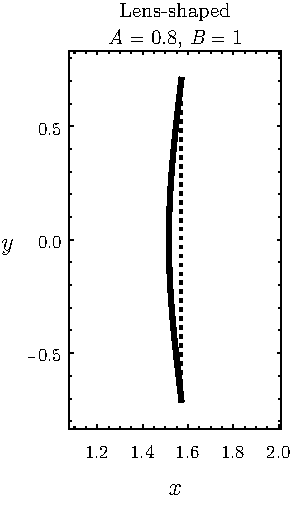
\includegraphics[height=0.6\textwidth]{cosine-verification-lens-domain}
  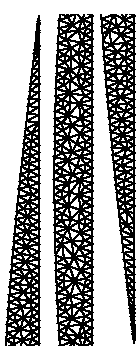
\includegraphics[
    width=0.16\textwidth,
    trim=0 {-\legendoffsetheight} 0 0,
  ]{cosine-verification-lens-mesh}
  \hfill
  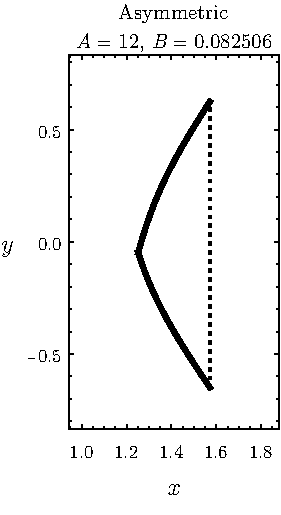
\includegraphics[height=0.6\textwidth]{cosine-verification-asymmetric-domain}
  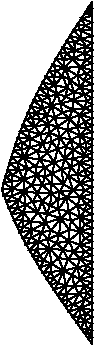
\includegraphics[
    width=0.11\textwidth,
    trim=0 {-\legendoffsetheight} 0 0,
  ]{cosine-verification-asymmetric-mesh}
  
\includegraphics[width=\textwidth]{cosine-verification-legend}
  \caption{
    Selected domains and finite element meshes for numerical verification.
  }
  \label{fig:cosine-verification-domain-meshes}
\end{figure}

Figure~\ref{fig:cosine-verification-domain-meshes}
shows the two selected test domains:
for the simple case~($B = 1$),
this is the lens-shaped domain with~$A = 0.8$,
and for the general case~($B$~arbitrary),
the asymmetric domain constructed
in Figure~\ref{fig:cosine_general-asymmetric_domain}.
Each domain is discretised into an unstructured triangular mesh
with around 500~elements.

\begin{figure}
  \newcommand*{\subfigurewidth}{0.42\textwidth}
  \centering
  \hspace*{\fill}
  \begin{subfigure}[t]{\subfigurewidth}
    \centredfigurecontent[trim=0 -1 0 0]{%
      cosine-verification-lens-relative-error%
    }{%
      Lens-shaped
    }
  \end{subfigure}
    \hfill
  \begin{subfigure}[t]{\subfigurewidth}
    \centredfigurecontent{%
      cosine-verification-asymmetric-relative-error%
    }{%
      Asymmetric
    }
  \end{subfigure}
  \hspace*{\fill}
  \caption{
    Relative error of numerical solutions computed in the selected domains.
  }
  \label{fig:cosine-verification-relative-error}
\end{figure}

\begin{figure}
  \newcommand*{\subfigurewidth}{0.36\textwidth}
  \centering
  \hspace*{\fill}
  \begin{subfigure}[t]{\subfigurewidth}
    \centredfigurecontent[trim=0 -1 0 0]{%
      cosine-verification-lens-relative-error-histogram%
    }{%
      Lens-shaped
    }
  \end{subfigure}
    \hfill
  \begin{subfigure}[t]{\subfigurewidth}
    \centredfigurecontent{%
      cosine-verification-asymmetric-relative-error-histogram%
    }{%
      Asymmetric
    }
  \end{subfigure}
  \hspace*{\fill}
  \caption{
    Histogram of relative errors
    evaluated at the finite element mesh nodes
    for the selected domains.
  }
  \label{fig:cosine-verification-relative-error-histogram}
\end{figure}

Laplace's equation~(\ref{eq:laplace-steady-conduction}) is then solved,
with the radiation condition~%
  (\ref{eq:cosine-scaled-radiation-boundary-condition})
applied along the radiation boundary
and the Dirichlet condition~$T = 1$ applied
along the constant-temperature boundary~$x = \pi/2$.
The agreement between the resulting numerical solutions
and the exact solution~(\ref{eq:cosine-scaled-laplace-solution})
is excellent.
In both cases the relative error is strictly less than~$7 \times 10^{-4}$
throughout all nodes of the mesh,
with the largest error realised at the two corners
where the radiation boundary meets the constant-temperature boundary
(Figure~\ref{fig:cosine-verification-relative-error}).
Moreover,
the bulk of the relative error is in fact much smaller than this,
as can be seen from the histograms
in Figure~\ref{fig:cosine-verification-relative-error-histogram}.
We can therefore be completely confident
in the validity of the boundary tracing procedure.

\section{Summary}
\label{sec:cartesian.summary}

In this chapter we have applied the method of boundary tracing
for the conduction--radiation problem in Cartesian coordinates.
Starting from the simplest possible solution,
namely the one-dimensional solution~(\ref{eq:plane-laplace-solution}),
we have produced
a family of hypergeometric traced boundaries
with translational symmetry in~$y$.
By construction
the radiation condition~(\ref{eq:radiation-boundary-condition})
holds exactly along these boundaries,
and they may be patched together
to form a broad variety of radiation boundaries.
Unfortunately these boundaries are not convex,
which is problematic
since the boundary condition~(\ref{eq:radiation-boundary-condition})
does not account for self-viewing radiation.
Nevertheless, we have shown how to identify near-convex fins
for which the amount of self-viewing radiation is negligible.
Returning to physical (unscaled) variables,
we have constructed an explicit example of a fin
whose length and temperature are of a practical scale.

Seeking a more favourable outcome with respect to convexity,
we have also started from
the cosinusoidal solution~(\ref{eq:cosine-laplace-solution}),
which is not one-dimensional.
In the simple case~($B = 1$)
we have seen that a convex, lens-shaped domain can be produced
when the dimensionless group~$A$ belongs to a certain interval.
We have then extended this interval
so as to obtain near-convex domains
having only a small amount of self-viewing radiation.
For the more complicated general case~($B$~arbitrary)
we have demonstrated the construction of an asymmetric domain
from convex portions of the traced boundaries.
Finally the validity of the domains produced has been confirmed,
by comparing numerical solutions for the conduction--radiation BVP
(obtained using the finite element method)
with the exact cosinusoidal solution
we started with.
